\documentclass{article}

\usepackage[latin1]{inputenc}
\usepackage[brazil]{babel}
\usepackage{graphicx}
\usepackage{xcolor}
%\usepackage{hyperref}

\begin{document}

\section{Primeira Se��o}\label{sec01}
Lorem ipsum dolor sit amet, consectetuer adipiscing elit. 

\begin{figure}[h]
	\centering
	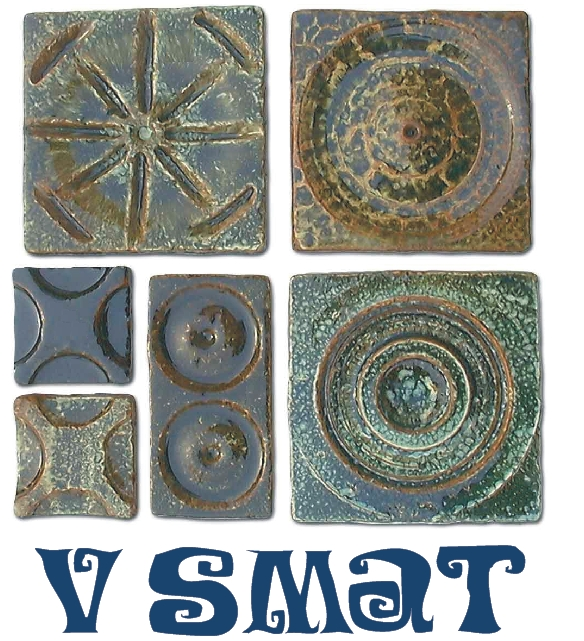
\includegraphics[scale=0.2]{vsmat.jpg}
	\caption{Este � o logo do SMAT 2010!}
	\label{smat}
\end{figure}

Ut purus elit,
vestibulum ut, placerat ac, adipiscing vitae, felis. 
Referenciando a figura \ref{unesp}! Curabitur dictum 
gravida mauris. Nam arcu libero, nonummy eget, consectetuer 
id, vulputate a, magna. Donec vehicula augue eu neque.

Agora vamos fazer a refer�ncia � se��o \ref{sec02}.

\section{Segunda Se��o}\label{sec02}
Pellentesque habitant morbi tristique senectus
et netus et malesuada fames ac turpis egestas. 
Mauris ut leo. Cras viverra metus rhoncus sem. 

\begin{figure}[h]
	\centering
	
\includegraphics[scale=0.3]{unesp_3D.png}
	\caption{Voc� reconhece esta imagem?}
	\label{unesp}
\end{figure}

Nulla et lectus vestibulum urna fringilla ultrices. 
Phasellus eu tellus sit amet tortor gravida placerat. 
Integer sapien est, iaculis in, pretium quis, viverra 
ac, nunc. Praesent eget sem vel leo ultrices bibendum. 
Aenean faucibus. Morbi dolor nulla, malesuada eu, pulvinar 
at, mollis ac, nulla. 

Curabitur auctor semper nulla. Donec varius orci eget risus. 
Duis nibh mi, congue eu, accumsan eleifend, sagittis quis, 
diam. Duis eget orci sit amet orci dignissim rutrum. 

Vamos fazer refer�ncia � se��o... \ref{sec01}.

A imagem do smat est� na se��o \ref{smat}. 
Agora vamos mostrar em que p�gina ela est�, \pageref{smat}.

\begin{figure}[h]
	\centering
	
\includegraphics[scale=0.7]{logo.pdf}
	\caption{Voc� reconhece esta imagem?}
	\label{unesp2}
\end{figure}


\end{document}